%POLAR COORDINATES
%The print template for A4 paper (portrait)
%Author: Zoran Nikolic
% http://www.texample.net/tikz/examples/polar-coordinates-template/
\documentclass[12pt]{article}
\usepackage[margin=0.5in,paper=a4paper]{geometry} %Shrinking margins to 0.5in
\usepackage[x11names]{xcolor}                     %Additional colors
% TikZ graphivc language is described in: http://cremeronline.com/LaTeX/minimaltikz.pdf
\usepackage{tikz}
% For the numeric value calculation look this link: https://tex.stackexchange.com/questions/337831/pgfmathparse-basic-usage

\begin{document}
\thispagestyle{empty} %Please, no page numbers or similar
{\fontfamily{lmss}\selectfont
\begin{center}
    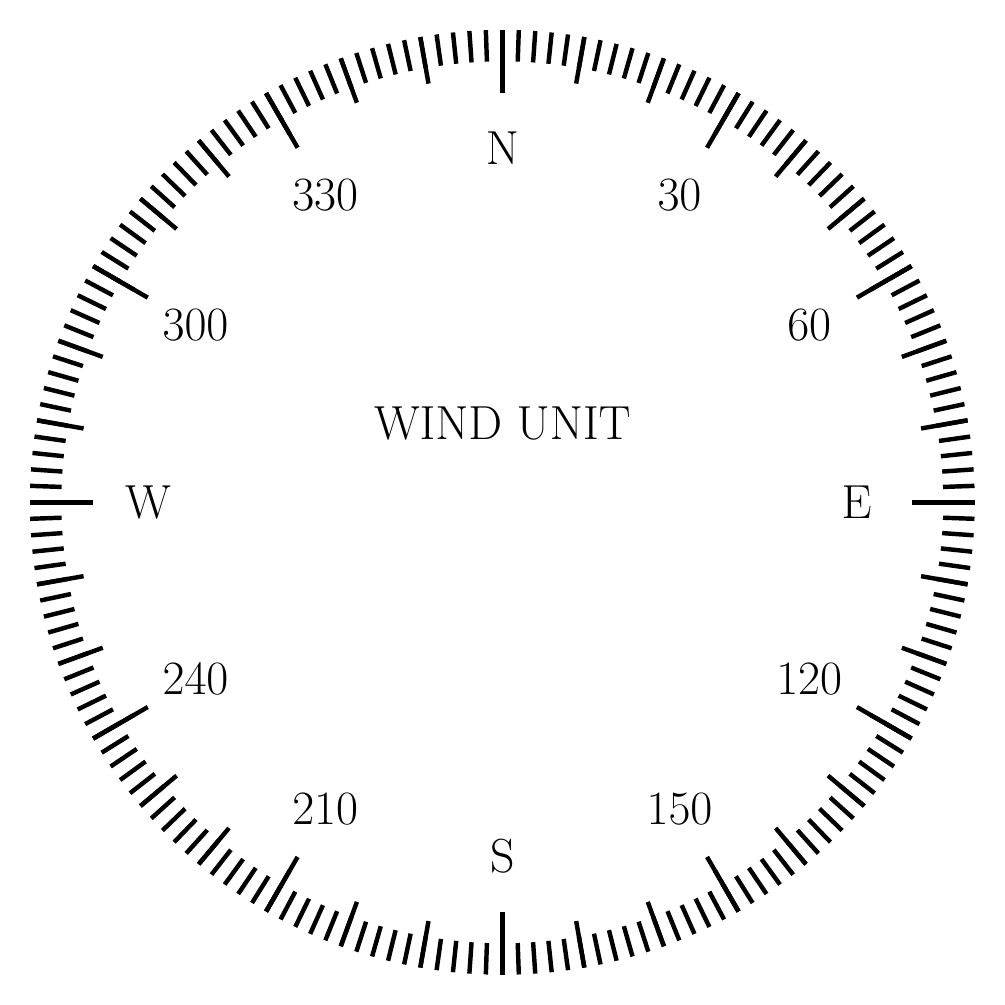
\begin{tikzpicture}
            %1° Rays
        \foreach \a in {0, 2,...,359}
        \draw[ultra thick] (\a:5.6) -- (\a:6);
            %5° Rays
        \foreach \a in {0, 10,...,359}
        \draw[ultra thick] (\a:5.4) -- (\a:6);     
            %10° Rays
        \foreach \a in {0, 30,...,359}
        \draw[ultra thick] (\a:5.2) -- (\a:6);
            %Angle labels 
        \foreach \a in {30, 60, 120, 150, 210, 240, 300, 330}
                \pgfmathtruncatemacro\result{360 - \a}
        \draw (\a + 90: 4.5) node {\LARGE\result};
        \foreach \a in {0}
        \draw (\a + 90: 4.5) node {\LARGE{N}};
        \foreach \a in {270}
        \draw (\a + 90: 4.5) node {\LARGE{E}};
        \foreach \a in {180}
        \draw (\a + 90: 4.5) node {\LARGE{S}};
        \foreach \a in {90}
        \draw (\a + 90: 4.5) node {\LARGE{W}};
        \draw (90:1) node {\LARGE{WIND UNIT}};
    \end{tikzpicture}
\end{center}
}
\end{document}
